\newcommand{\pintosenvfigure}{
    \begin{figure}[htp]
    \centering
    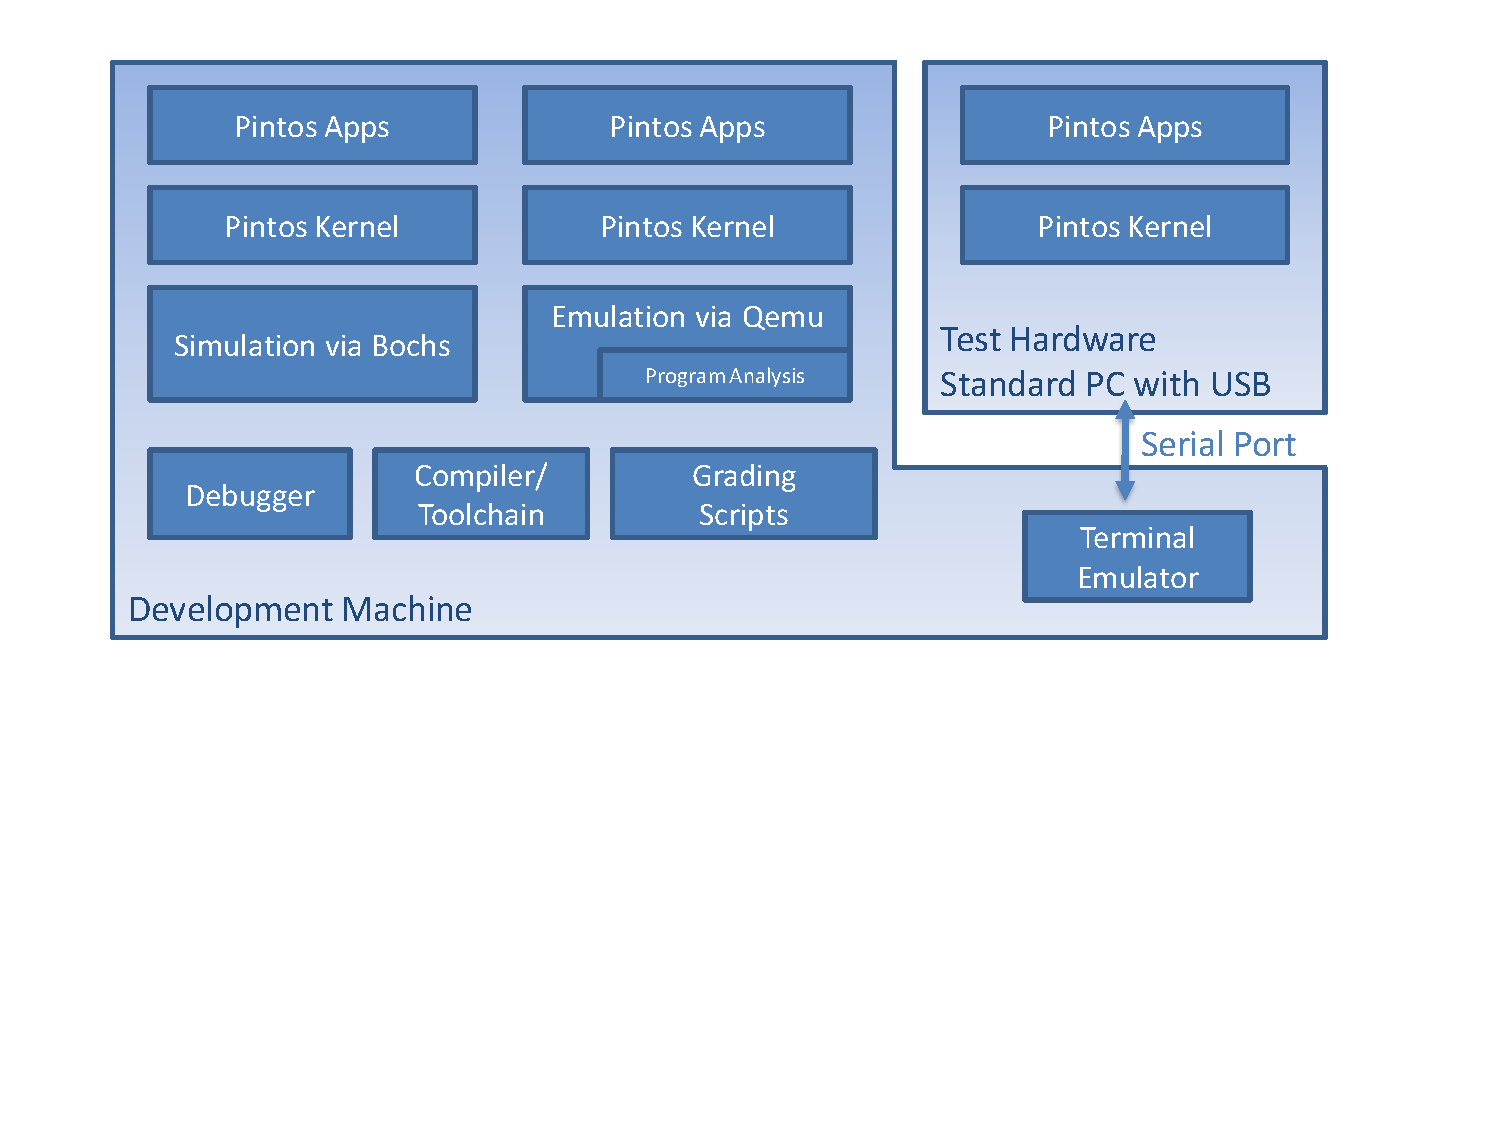
\includegraphics[trim=.5in 3.2in .7in .3in, clip,width=\columnwidth]{pintosoptions.pdf}
    \caption{The same Pintos instructional kernel runs in a
    fully reproducible simulated environment, in an enhanced
    emulated environment with dynamic analysis capability, and
    on actual hardware.}
    \label{fig:pintosenvs}
    \end{figure}
}

\newcommand{\pintosdetailfigure}{
    \begin{figure*}[htp]
    \centering
    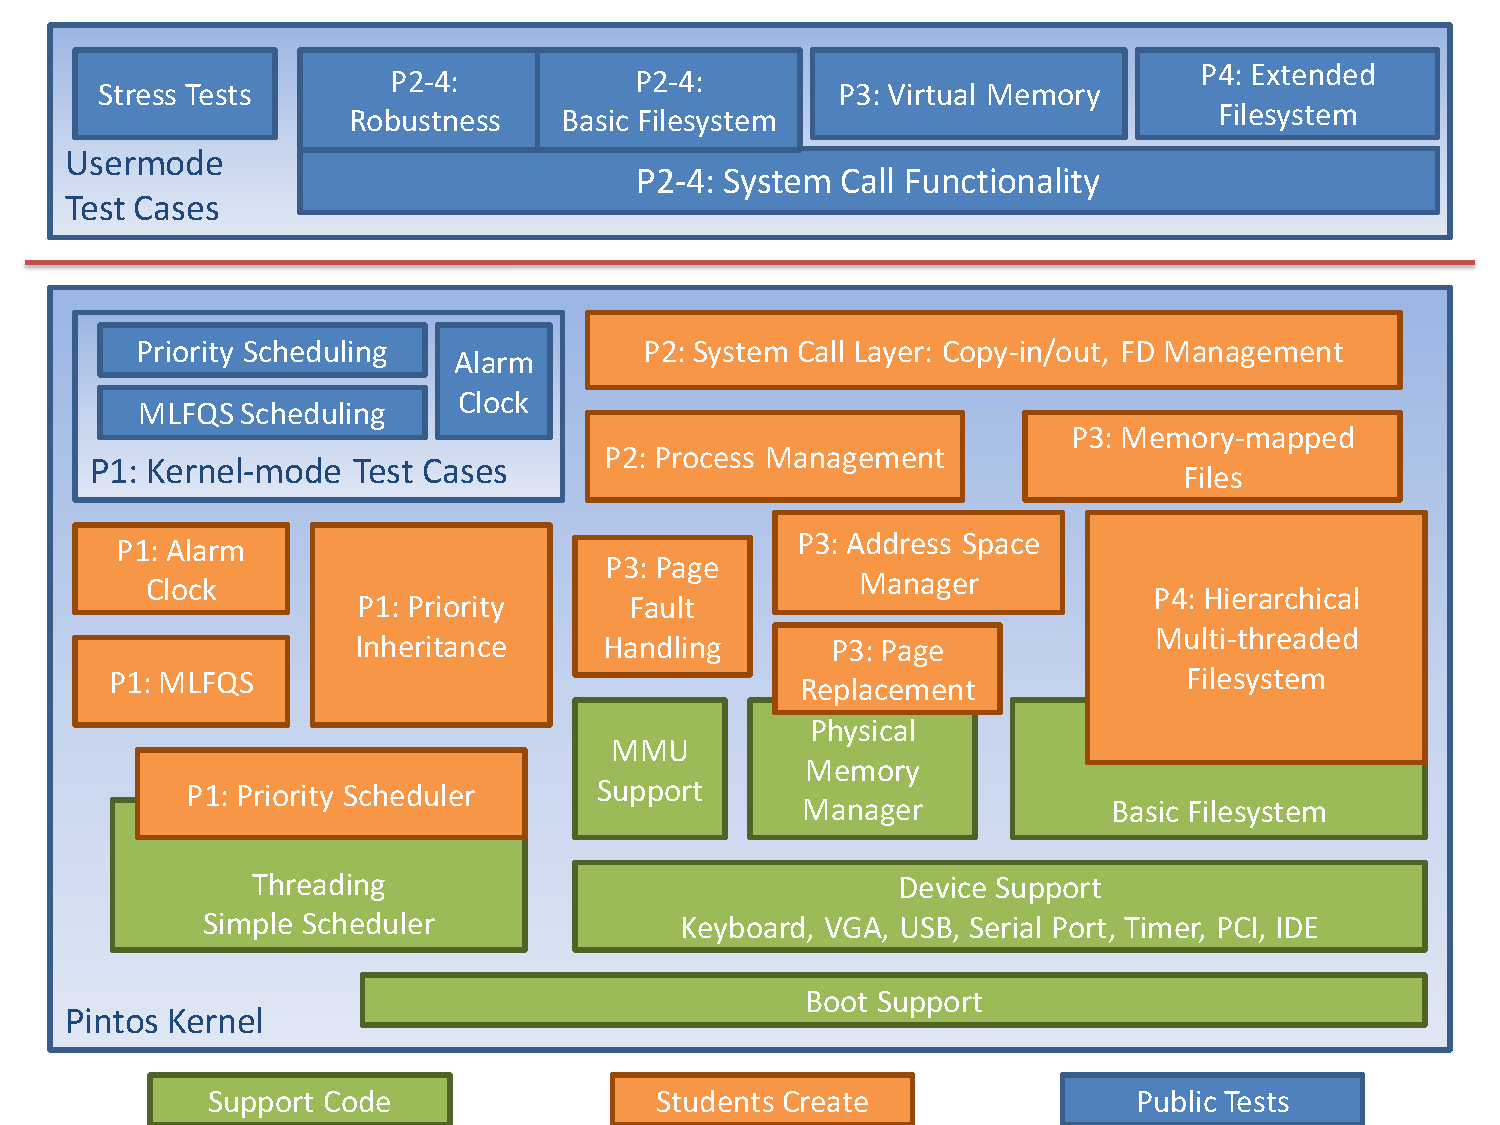
\includegraphics[width=.7\textwidth]{pintosoverview.pdf}
    \caption{Components of Pintos split in provided support code, test cases, 
        and components created in assignments.  Overlapping components indicate
        when students have to replace parts of the support code.}
    \label{fig:pintosdetail}
    \end{figure*}
}

\newcommand{\pintostestcounttable}{
\begin{table}
    \begin{tabular}{lccc}
    Project & Functionality & Robustness & Regression \\
    1       & 27            & -          & -          \\
    2       & 41            & 35         & -          \\
    3       & 20            & 14         & 75         \\
    4       & 39            & 7          & 75         \\
    \end{tabular}
    \caption{Pintos test cases by project.}
    \label{table:tests}
\end{table}
}
